%!TEX root = ../report.tex

\begin{document}
  \chapter{Experimental Setup}

  Having applied the theoretical knowledge derived in Section 3 to the ROPOD case
  study in Section 4 we have begun to narrow down the options for spatio-temporal
  world modeling in this particular case. However, a theoretical comparison will
  only suffice for so long. Given the focus ROPOD places on real world
  environments it is critical that some operational tests be preformed before
  method selection. Not only will these experiments serve as a guide for ROPOD,
  but they will also act as a template for the comparison of future
  spatio-temporal world modeling techniques. \\

  \section{ Environmental Representation}

  Given the complexity and size of the target environment for ROPOD, a large
  hospital, it is necessary to pair down features of the building until only
  the core components remain. The three dynamic environmental components being
  target are doors, path planning with carts that are often strewn about the
  hallways and surrounding rooms, and elevators. Therefore, a model
  environment has been designed for the simulations to be run on that contains
  these three key components.  The model environment that has been designed
  takes heavy influence from the actual environment but some notable have been
  made. The model has a decreased area to allow for faster model training and
  path planning. Additionally, extraneous rooms and hallways have been
  removed. A comparison between the actual hospital and the designed model can
  be seen below.

  TODO add picture


  \section{ Common Assumptions }
  In order to insure only the desired component is being tested at any given
  time a set of assumptions are made.

  \begin{itemize}

    \item All robot components are working correctly (no internal faults)

    \item Other than the object under test (e.g. doors), all other objects in the
          environment are static

    \item All information other than the objects under test are perfectly known

    \item Observations made/provided by the training data are assumed to be
          ground-truth

  \end{itemize}


  \section{ Commonalities in Approach }
  Although different components will be under test, each experiment will be run
  in a similar manor.

  The experimental setup is as follows:

  \begin{itemize}

    \item Training data consisting of observations made every 15 minutes over
          a simulated month will be provided to the models

    \item All data generation will be done using the same program and the
          specifics of how the data is generated will be discussed further
          below in the relevant experiment section

    \item Using the same generation procedure, a new month will be generated

    \item The models will be trained using the original month and then tested
          against both the original month and the new test month

    \item In the case of the doors and elevator, only the objects themselves
          will be modeled and the comparison will only be how well the generated
          models can predict the ground thruth

    \item In the case of the more advanced hallway scenario, predictions about
          objects in the environment will be used to plan a path and this path
          will be compared with paths planned using the ground truth

    \item All of these paths will then be compared using the criteria described
          below.

    \item All experiments will be done on the same hardware
      \begin{itemize}
        \item ASUS UX330UAK Laptop
        \item i5-7200k 2.5GHz
        \item 8GB DDR3
        \item Arch Linux 4.19.4
      \end{itemize}

  \end{itemize}

  \section{ Data Generation }

  Data generation is done using a combination of built in Python libraries and
  the NumPy library. Each object is broken down into a series of days which is
  then further broken down into a series of behaviors. Each behavior
  represents the likelihood of an object being in a given state between two
  times.  Furthermore, each behavior has a starting state and an ending state,
  which if different, are swept through linearly. E.g. if a behavior is
  modeling a binary state of a door that starts at 100\% open and then becomes
  100\% closed an hour later at the half hour mark the door would have the
  door being at a 50\% likelihood of being open. Additionally, it is possible
  to specify the amount of Gaussian noise that is added on top of the
  behavior where the nominal state is used as mu and the sigma is used to
  specify the magnitude of the noise. Months of data are thus generated by
  walking through these behaviors in 15 minute increments for each day in the
  month where each month is assumed to have exactly 31 days. \\

  For example, if a door was open from noon until midnight every day, and then closed from
  midnight until noon there would be two behaviors one from midnight until
  noon and one from noon until right before midnight. In this case, the
  starting and ending values of each behavior would be the same and no noise
  would be introduced. This would create a sharp, well defined change at
  exactly noon and midnight every day. Further details and specifics about data
  generation will be discussed in their respective sections. \\

  \section{ Model Parameters }
  TODO expand? \\

  Four models will be tested: Duckett's TODO, FreMEn, HyperTime, and Gaussian
  Mixture Models. HyperTime and FreMEn are of particular interest as they will
  be able to represent non-binary states. HyperTime will be using the
  expectation mean variant TODO why? The Gaussian Mixture Model, despite not
  being expected to preform as well as the others, has been included as a
  comparison with previous experiments like that done in TODO SITE. FreMEn and
  HyperTime will both use an order of three as that has, on average produced,
  the best results as seen in TODO SITE and improve Duckett info. During
  non-binary prediction HyperTime requires an upper limit for it estimates. In
  the case of the elevator experiment, an upper limit of 30 (seconds) has been
  given. This will be expanded upon in Section 6. The Duckett approach will
  contain three sub-models. The models will have a TODO wording .75, .25, and
  .05 TODO replacement rate? all with a size of 20. This is to closely match
  the approach in TODO PAPER. The three internal models will be averaged
  together to produce a prediction.\\

  It is important to note that unlike the other three approaches, Duckett does
  not inherently support the ability to predict events arbitrarily in the future.
  It is limited to a single immediate prediction. Therefore, future predictions
  will done by simply projecting historical predictions forward on a monthly basis.
  That is to say, whatever Duckett's prediction was on the third of the first month
  it will be the same on the third of the next month. \\

  The Duckett implementation was done using Python 3 while Gaussian Mixture
  Models, FreMEn, and HyperTime were all written in C++. The Duckett implementation
  was written by the author of this paper TODO phrasing? while the other three
  are available on Tom Krajnik's Github page. TODO link? Finally, the non-binary
  version of HyperTime, although not currently freely available on Github, can
  be obtained upon request as mentioned in the binary only repository.




  \section{ Comparison Criteria }
  In order to evaluate the intricacies of the selected models a wide variety
  of data points have been selected for comparison. A focus has been placed on
  collecting data relevant to accuracy and scale-ability of the modeling
  technique given the eventual scope of the ROPOD project.

  \begin{itemize}

    \item Accuracy to Ground Truth

    \item Accuracy to Historical Recreations

    \item Planning Run-time

    \item Planning Memory Consumption

  \end{itemize}

  \section{ Doors as Dynamic Objects }

  \subsection{ Experimental Motivation }

  As is the case in many places of employment many areas of a building may not
  be accessible to the public, and by extension the robots, outside of work
  hours.  This could come in the form of a given hallway between two areas being
  locked after 17:00 as the day works go home. In another case, it could be as
  simple as someone preferring to having a door shut to a hallway during a loud
  or chaotic time of the day. \\

  Regardless of the reason, it is certain that the states of doors are often
  both dynamic exhibiting both periodic and long term changes. In the ideal case, a robot, much like humans,
  would learn when certain doors are closed and be able to plan accordingly.
  Making an accurate prediction can save time, but making an inaccurate
  predication can also be costly. An in accurate prediction would force a robot
  to not only backtrack, but also recalculate that path required to get to a
  target. Additionally, it may not be possible to make deliveries at all times.
  In the worse case, a robot may even manage to get itself locked in an
  environment unable to return back to it's base and eventually run out of power
  requiring human intervention. For these reasons and many more, the door
  experiment is an excellent example of the benefits of spatio-temporal world
  modeling. \\

  \subsection{ Experimental Details }

  In order to keep this test as straight forward as possible, only the door
  object itself has been modeled. The doors could belong to a room where a
  package must delivered or perhaps a hallway that could be used as a
  shortcut. Each model will be directly, or indirectly be tasked with
  predicting the state of this door. Figure 5.1 displays an example of three
  doors in ward 24 of the hospital that may display the dynamic behavior
  previously mentioned. \\

  When evaluating the predictions made by the models a simple 50\% confidence
  value will be used. That is to say, if a model predicts that the door will
  be 50\% or more likely to be open will result in the robot attempting to
  deliver the package. \\

  \begin{figure}[!htb]
    \centering
    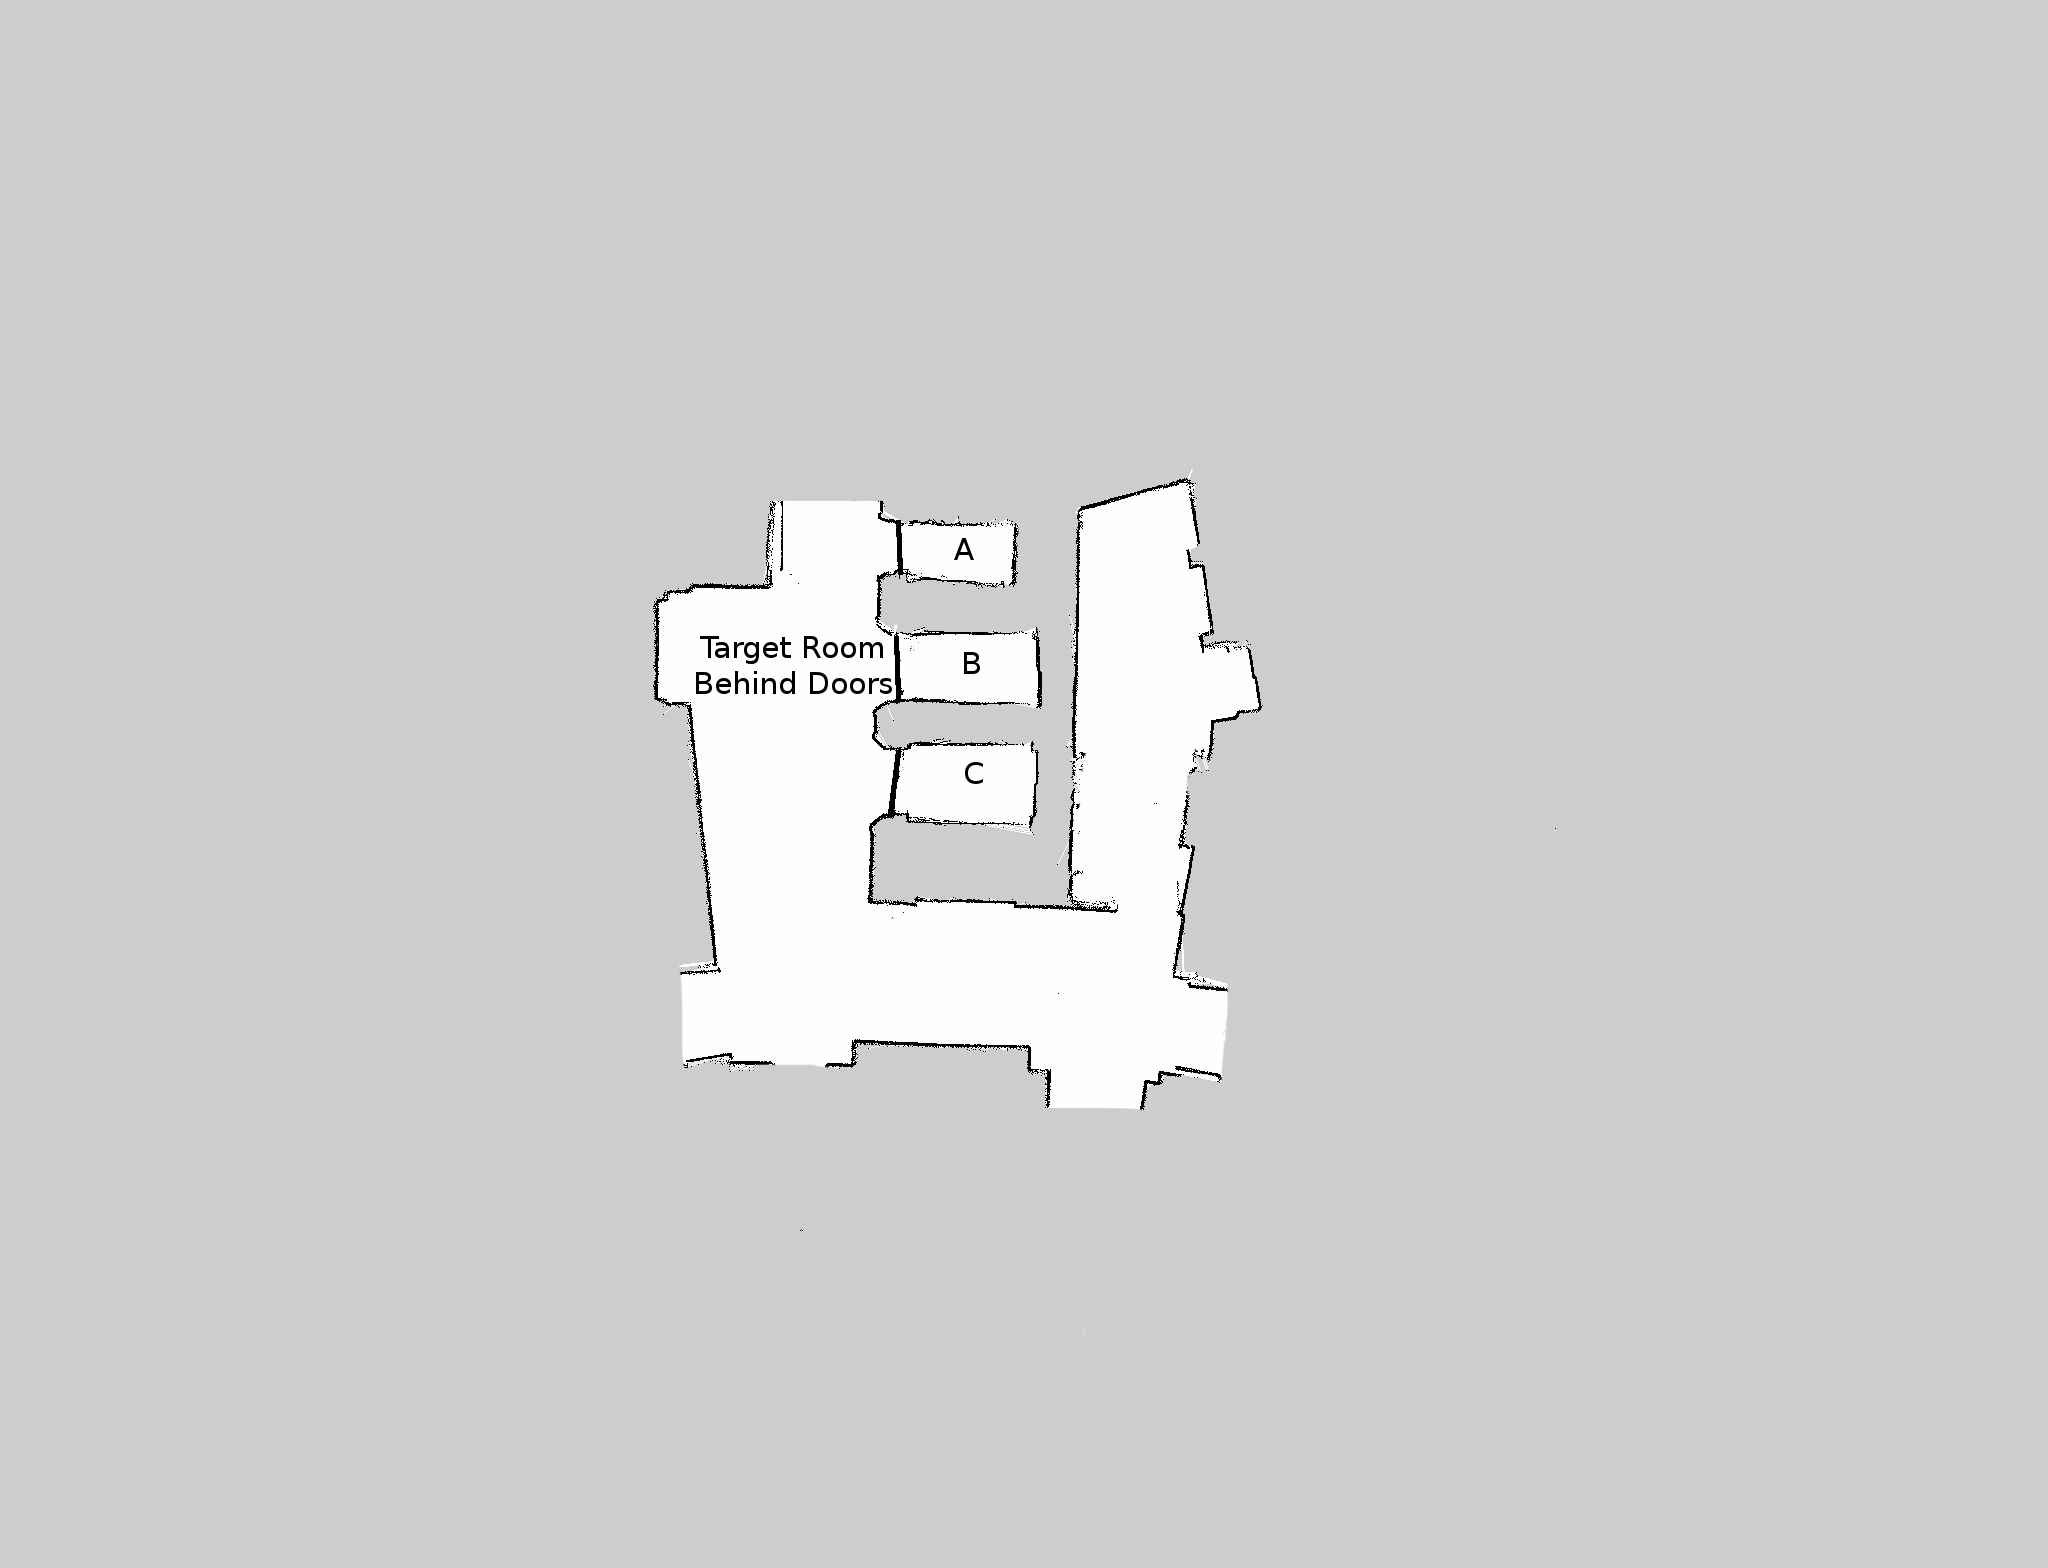
\includegraphics[width=\linewidth]{images/ward_24_door.png}
    \caption{Multiple rooms behind doors in ward 24.}
    \label{figure:ward_24_door}
  \end{figure}

  It is clear that this 50\% cutoff does not take into account the penalties
  of making a wrong prediction, but this particular experiment was designed to
  investigate the accuracy of the prediction. The hallway experiment discussed
  below will delve a little deeper into the ramifications of inaccurate
  predictions. That being said, how the information of the prediction is
  handled afterwards is undoubtedly valuable, but is outside the scope of this
  current research.

  \subsection{ Data Generation }

  As mentioned above, both the training and the test data for all models was
  generated using the same program.

  The specifics for each door are as follows.

  \subsubsection{ Door A }

  Door A is models a door that is highly influenced by the daily schedule of a
  9:00 to 17:00 job and has a high amount of periodic behavior with a small
  amount of noise.  There are 5 behaviors which model a standard work day. The
  time from midnight until work starts at 9 has the door in a normally closed
  state.  From 9:00 until 12:00 the door is likely open. 12:00 until 13:00 is
  considered lunch time and thus the door is likely closed. Work resumes at
  13:00 until 17:00 and thus likely open. From 17:00 until midnight
  the door remains in a likely closed state. Finally, the door is always
  closed on weekends with a 100\% probability and no noise. \\

  When the door is in a likely open state it has 70\% chance of being open.
  Likewise, when in a likely closed state it has a 70\% chance of being closed.
  Finally, when noise is introduced during the weekday it uses a standard deviation
  of 0.1 where mu is either 0.3 or 0.7 and 0.5 is the cutoff for being open or
  closed. \\

  \begin{figure}[!htb]
    \centering
    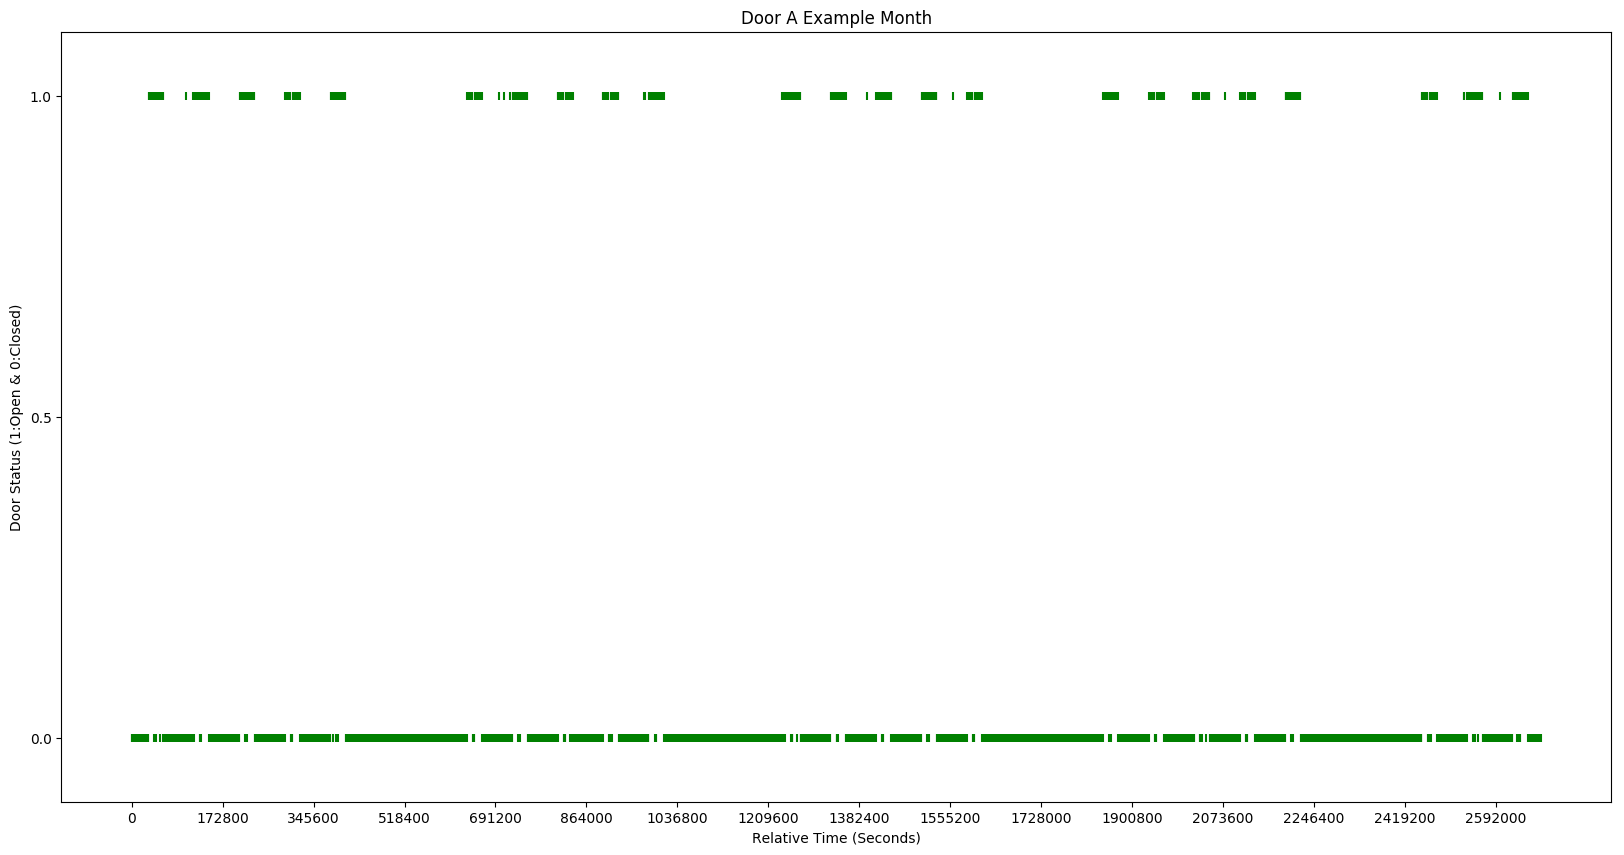
\includegraphics[width=\linewidth]{images/Door_A_Example_Month.png}
    \caption{The training data for Month A}
    \label{figure:Door A Training Month}
  \end{figure}

  \subsubsection{ Door B }

  Door B, in a similar manor to door A, also tries to encapsulate the periodic
  behaviors of a work day but with a little more noise. Door B is always open
  from midnight until the start of the work day at 9:00. During the work day
  the door is a constant state of flux, being open and shut at random. This is
  modeled using a mu of 0.5 and a standard deviation of 0.1. This ends when
  the work day is over at 17:00 and the door goes back to remaining open until
  the next work day starts. To add additional periodic complexity, such as a
  weekly meeting or delivery, every third weekday the door will be closed the
  entire day. This trend is continued across month boundaries. This means if
  the doors was closed on the day before the last day of the first month it
  will again be closed on the second day of the next month. Finally, on
  weekends the door will always be open with 100\% certainty and no noise. \\

  \begin{figure}[!htb]
    \centering
    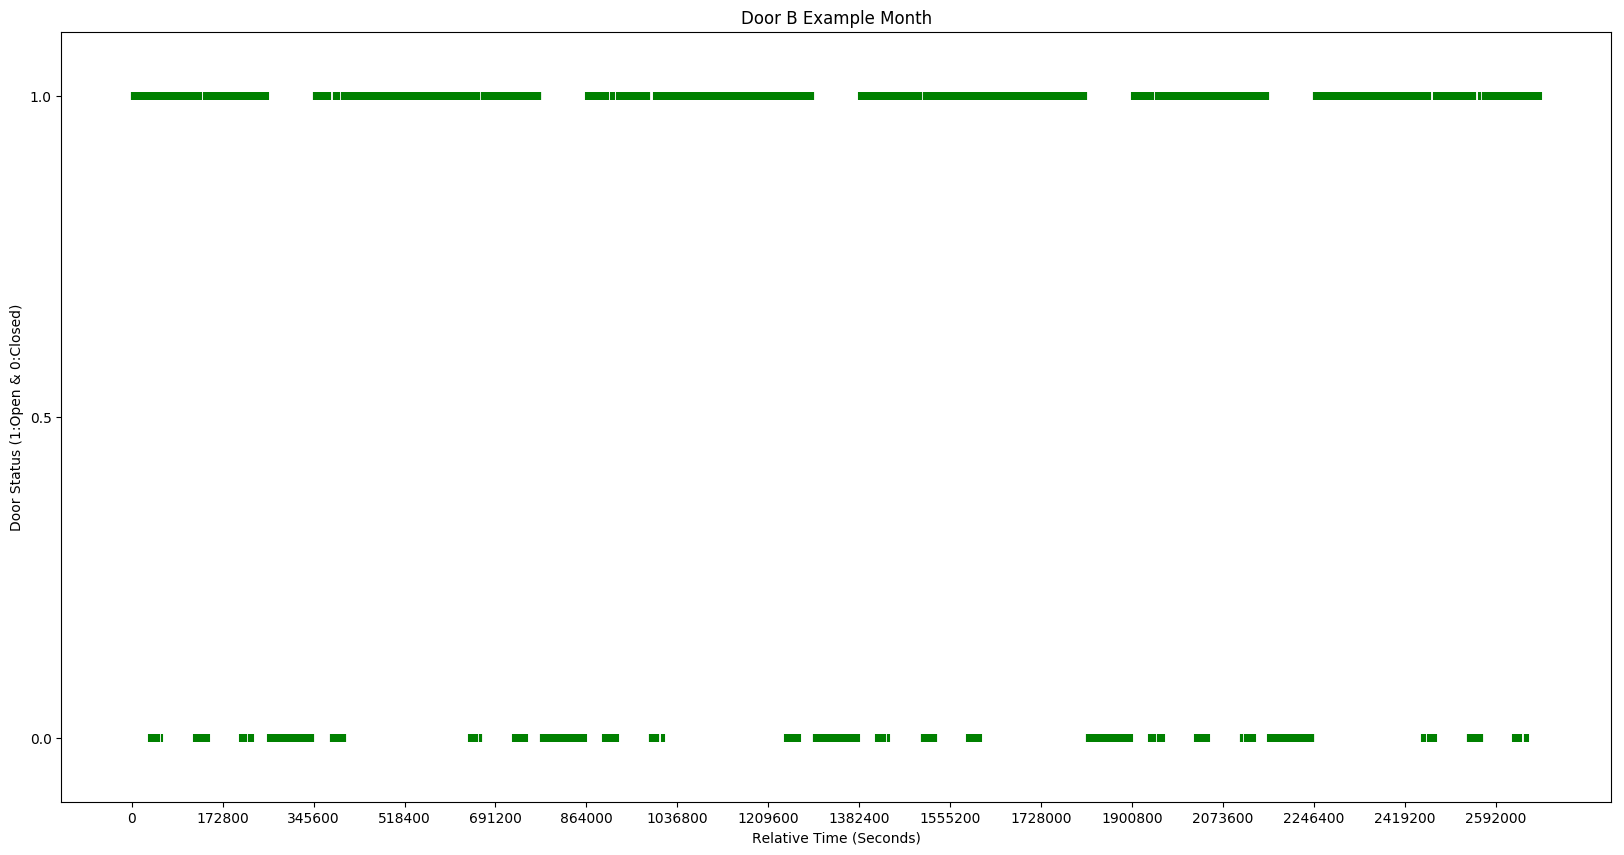
\includegraphics[width=\linewidth]{images/Door_B_Example_Month.png}
    \caption{The training data for Month B}
    \label{figure:Door B Training Month}
  \end{figure}

  \subsubsection{ Door C }

  Door C does not attempt to model any periodic behavior but instead test
  long-term change in an environment. A simple illustration of the long-term
  non-periodic change could be that of construction. The door has always been
  open in the past but it leads to a wing of the building that is now either
  being remodeled or has been removed. In the test data, this behavior is
  achieved by having the door be open for the first three weeks and then being
  closed for the rest of the training month and through the test month. In
  this model no noise was introduced. \\

  \begin{figure}[!htb]
    \centering
    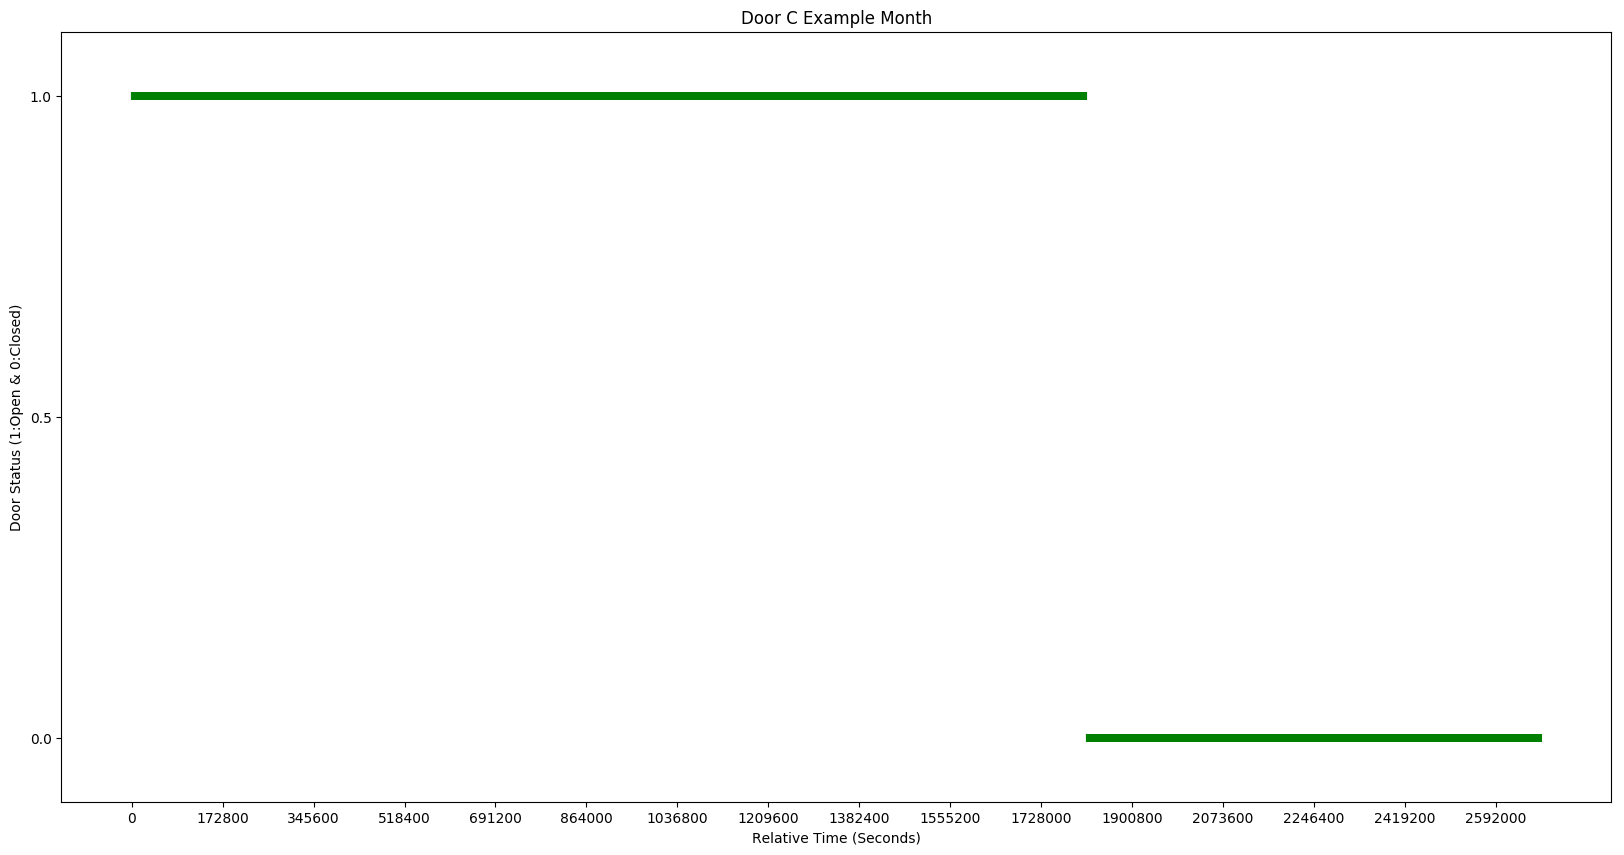
\includegraphics[width=\linewidth]{images/Door_C_Example_Month.png}
    \caption{The training data for Month C}
    \label{figure:Door C Training Month}
  \end{figure}


  \clearpage
  \section{ Path Planning in Congested Hallways}

  \subsection{ Experimental Motivation }

  Individual object representation and performance is vital for initial
  evaluation of an algorithm, but more expansive test must be completed to
  build a complete picture of an algorithms real-world performance. It is for
  this reason multiple dynamic objects will be used to model an environment
  that closely replicates that of ROPODs target environment. Not only does this
  serve as an excellent test case for ROPOD but it also serves as an initial
  evaluation into the scalability of a method. \\

  When planning paths with multiple dynamic objects it is critical that not just
  few, but all of the objects are correctly predicted. If any of the objects state are
  predicted incorrectly a robot may need to reroute dynamically or in the worst
  case it may not be able to arrive at its destination at all wasting time and
  resources.


  \begin{figure}[!htb]
    \centering
    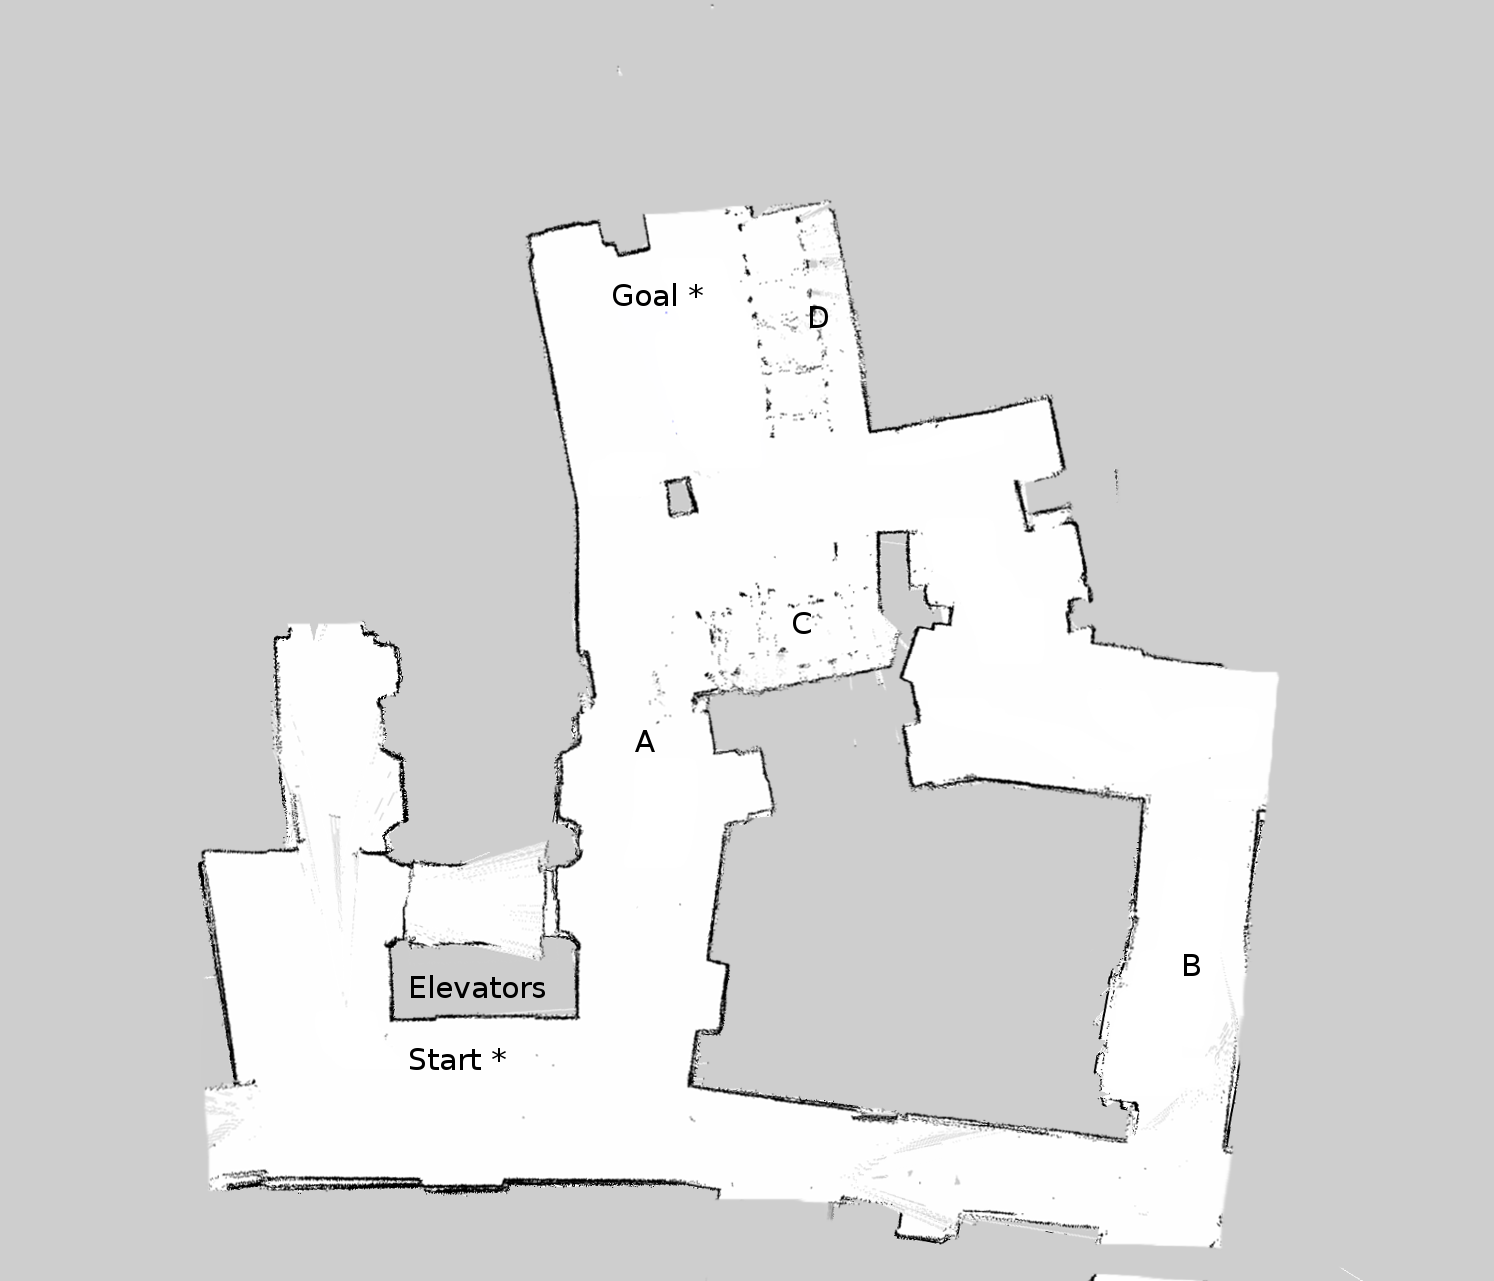
\includegraphics[width=\linewidth]{images/basement_congestion.png}
    \caption{The path from the elevator to the storage area is often congested with multiple dynamic obstacles. }
    \label{figure:basement_congestion}
  \end{figure}

  \clearpage


  \subsection{ Experimental Details }

  \begin{figure}[!htb]
    \centering
    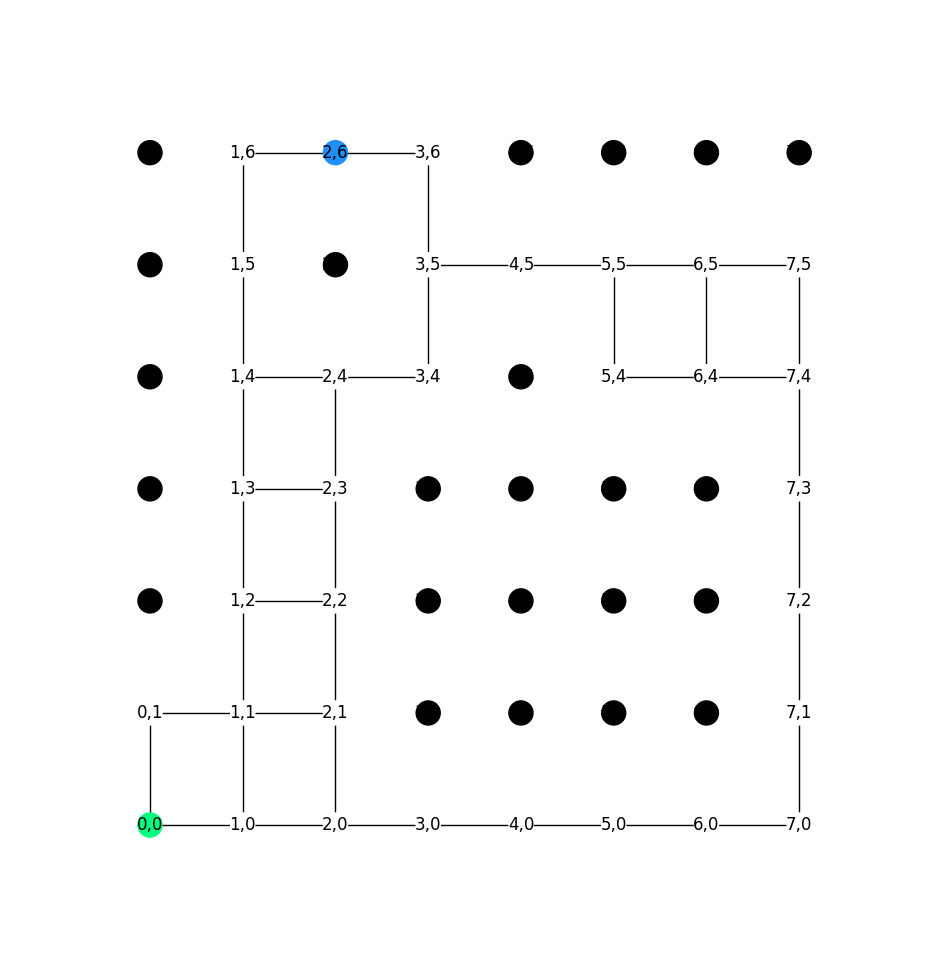
\includegraphics[width=\linewidth]{images/results/Empty_Hospital.png}
    \caption{Graph representation of the hospital basement with no obstacles}
    \label{figure:basement_congestion_empty}
  \end{figure}

  The specific area under test in this experiment is a representation
  of the basement area of the hospital ROPOD will be deployed in. Figure 5.5
  is a slightly cleaned up version of ROPOD generated map. Areas have been marked
  to highlight where common dynamic obstacles occur. Figure 5.6 shows a graph
  representation of this same area, simplified for path planning. Figure 5.7
  shows the same area but with all dynamic obstacles present. The obstacles
  and there frequencies are as follows: \\

  \begin{itemize}

    \item Meals - Three times a day

    \item Laundry - Once per day

    \item Delivery - Twice per week

    \item Trash - Once every three days

  \end{itemize}

  The edges in the graphs are the possible routes the robot is able to take.
  Node 0,0 represents the start state which is roughly where the robot would
  be after taking the elevator down. Node 2,6 is the goal state and represents
  an entrance into either a storage area or another hallway.

  \begin{figure}[!htb]
    \centering
    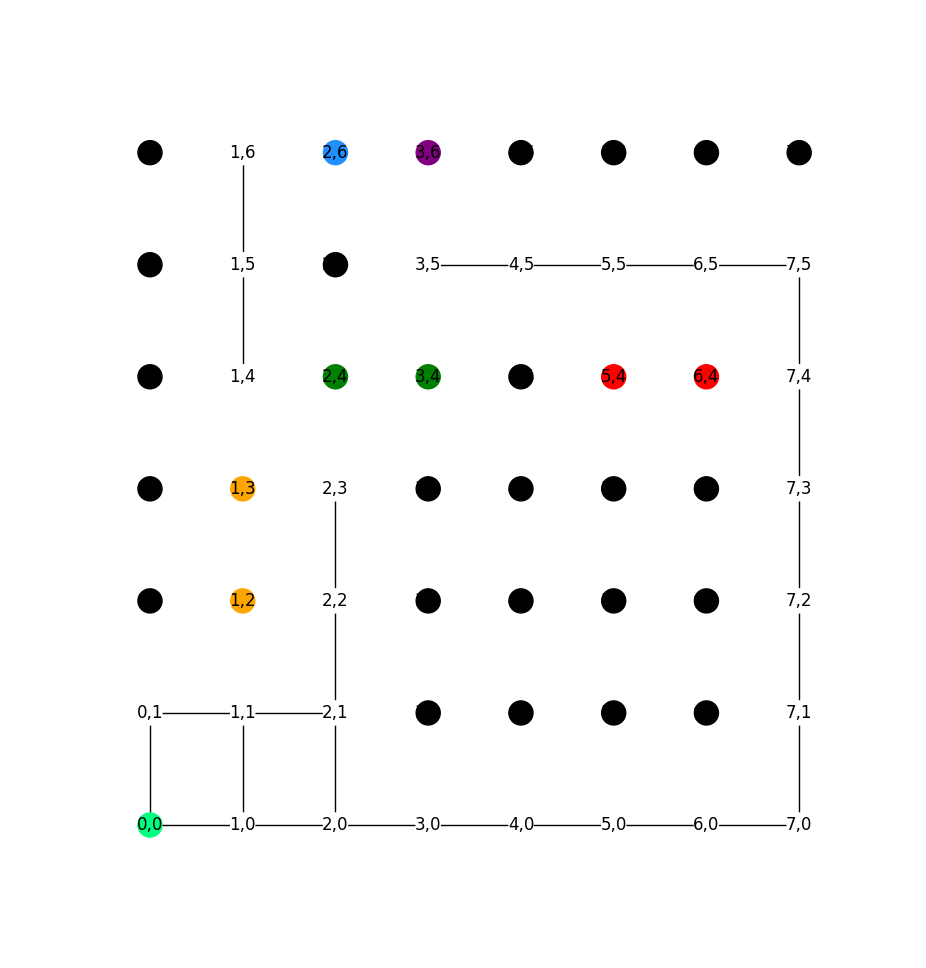
\includegraphics[width=\linewidth]{images/results/Full_Hospital.png}
    \caption{Graph representation of the hospital basement with all obstacles modeled}
    \label{figure:basement_congestion_full}
  \end{figure}



  \subsection{ Data Generation }

  The data for these test was generated using the same program as the doors
  and in the same manor. The graph generation and path planning was done using
  NetworkX a free and open source tool that allows for the creation and subsequent
  path planning on graphs amongst other functionality. More information can be
  found on there website at https://networkx.github.io/

  The specifics for each door are as follows.
  TODO perhaps a graph that shows all at once for a week?
  TODO where do I clarify that this is only for example and not real data again?
  TODO standardize order

  \subsubsection{ Meals - Nodes 1,2 \& 1,2}

  Meals are a periodic and consistent behavior in the hospital. They happen
  three times a day regardless of which day of the week it is. Meals and their
  respective dishes will be staged in the hallway before being moved to
  another area or delivered. For ease of simulation, carts begin to pile up
  at node 1,2 at 4:00 and continue to build up until overflowing into node 1,3
  at 6:00. These two nodes continue to be occupied until 8:00 when all carts
  are sent up for delivery once again making them free for traversal. The
  process repeats again starting at 12:00 and 16:00 using the same time steps.

  \subsubsection{ Laundry - Node 3,6 }

  Laundry, similar to meals, is assumed to build up periodically and daily
  causing node 3,6 to be blocked. Laundry is said to begin to build up slightly
  before midnight and begin causing a blockage at 00:00 until 12:00 at which
  point enough laundry has been processed that the node is again traversable.

  \subsubsection{ Deliveries - Node 5,4 \& 6,4 }

  Deliveries are assumed to happen twice a week, once on Monday and then again
  on Friday. For the sake of simulation, deliveries block nodes 5,4 and 6,4
  the entire day of the delivery, i.e. from 00:00 until 23:59.

  \subsubsection{ Trash - Node 2,4 \& 3,4 }

  Trash or other objects will periodically be temporally stored in the hallway.
  For the sake of simulation, trash is said to begin to build up at node 3,4
  and then expand into node 2,4. The first day of the first month, both nodes
  will be free for traversal. After the first day, at precisely 00:01 the first
  node is said to be blocked. After another day, the trash has grown large
  enough to block the second node. This cyclic behavior continues to happen
  when the second test month is generated. In summary, the first day both nodes
  are free, the second day the first node is occupied, the third both are
  occupied, and then on the forth day they are back to both being free for
  traversal.

  \subsubsection{ Areas of Particular Note }

  As visible in Figure 5.7 it is not always possible to reach the goal from the
  starting node. Additionally, certain obstacles also block paths that might
  normally be considered first. An example of this is the obstacles caused by
  the meal nodes which prevent to most direct path to the goal upon leaving
  the elevator. Choke points are also a concern. These happen when an obstacle
  or obstacles completely cut of a given path. Examples of this are when both
  laundry and the first trash node are present or when both trash nodes and both
  meal nodes are present.
  \clearpage





  \section{ Busy Elevators }

  \subsection{ Experimental Motivation }

  Historically, many efforts in the field of spatio-temporal world modeling
  have been focused on modeling or classifying behavior into one of two binary
  states. (TODO give some citations here) Although this works well of
  representing the traverseability of an environment or presence of an object,
  it does not translate well into the tracking and predicting the behavior and
  state of many real-world objects. The ability to track and predict
  non-binary behavior is particularly important when a robot shares an
  environment with humans. This could be tracking the density of people in an
  environment, the speed at which traffic flows, or any number of other
  non-binary variables that exist in a dynamic environment. \\

  With regards to ROPOD, an excellent example of this for is non-binary
  behavior is the necessity to use elevators to move goods about the hospital.
  Specifically, the time between calling an elevator and the actual arrive of
  the elevator may often appear random, but when observed throughout time
  it is possible to observe patterns in the wait time. In order to better
  optimize which elevator should be called or when a deliver should be made it
  is important to have accurate models for predicting this behavior.
  Additionally, although this information alone is useful, this concept can
  be applied to a multitude of areas within a dynamic human environment. \\

  \subsection{ Experimental Details }

  \subsection{ Adaption of Non-Binary Models }

  Two of the models being tested, HyperTime and Duckett, nativity support
  classification of non-binary data. Although FreMEn and Gaussian Mixture Models
  do not directly support the prediction of non-binary states, they have been
  modified in order to produce results for analysis. Before training either of
  the models, the data sets are ordered and split in half at the median. The
  median value is then used for classification. If an observed value is below
  the median it is a 0, whereas above would be a 1. In this way, a continuous
  dataset can be broken into two states. Predictions are then made as normal.
  In order to convert back to a non-binary value, each half of the split data
  set is averaged producing an average value for all values classified as 0 and
  all values classified as 1. This averages are then used for predictions. \\

  For example, if the original data set contained six observations,
  [1, 2, 3, 4, 5, 6] the dataset would be split into [1, 2, 3] and [4, 5, 6].
  Any prediction lower than four would be a 0 and higher a 1. All 0's during
  prediction would then be the average of the first dataset, e.g. 2 and all
  1's would result in a prediction of 5.

  \subsection{ Data Generation }

  As mentioned in the two previous sections, both the training and the test
  data for all models was generated using the same program. However, obviously
  due to the nature of the non-binary data, slight changes were made to be able
  to represent any set of arbitrary real numbers. Behaviors no longer represent
  the likelihood of an object being in one of two states, but instead, in this
  specific case, represent the average time one must wait after calling an
  elevator. There are still linear transitions between behaviors as well as
  a variable amount Gaussian noise being applied on top of the nominal state
  (i.e. noise applied on top of the average wait time). The month of training
  data is visible in TODO. \\


  \subsubsection{ Average Daily Model}
  In this particular simulation, ever day was treated as the same type of day
  for the month long simulations. Each day starts and ends with almost no wait
  time to simulate how infrequent the elevators are used during those times.
  Peak elevator use time, and thus peak delays, are said to occur around times
  when people would being arriving or leaving work or lunch. The specifics of
  the behaviors and their parameters are visible in Table
  \ref{table:elevator_day_t}. While ~\ref{figure:Elevator Training Data} show
  what an entire month of this data looks like.

  \begin{table}[!htb]
    \begin{tabular}{|l|l|l|l|l|}
      \hline
      Behavior Name          & End Time & Nominal Wait in Seconds (\mu) & Noise in Seconds (\sigma) & Max Wait \\ \hline
      Morning Lull           & 6:00     & 0                                 & 0.4                           & 2        \\ \hline
      Morning Early Arrivals & 7:30     & 0                                 & 0.5                           & N/A      \\ \hline
      Morning Pre Rush       & 8:30     & 2                                 & 2                             & N/A      \\ \hline
      Morning Work           & 10:00    & 9                                 & 1                             & N/A      \\ \hline
      Early Lunch            & 11:00    & 4                                 & 1                             & N/A      \\ \hline
      Lunch Pre Rush         & 11:30    & 4                                 & 2                             & N/A      \\ \hline
      Lunch Rush             & 12:30    & 9                                 & 2                             & N/A      \\ \hline
      Midday Work            & 13:30    & 9                                 & 1                             & N/A      \\ \hline
      Evening Pre Rush       & 16:00    & 4                                 & 2                             & N/A      \\ \hline
      Evening Rush           & 17:30    & 9                                 & 2                             & N/A      \\ \hline
      Day Wind Down          & 22:00    & 9                                 & 0.5                           & N/A      \\ \hline
      Day End                & 24:00    & 0                                 & 0.4                           & 2        \\ \hline
    \end{tabular}
    \caption{Behaviors used to describe daily wait times for the elevator}
    \label{table:elevator_day_t}
  \end{table}



  \begin{figure}[!htb]
    \centering
    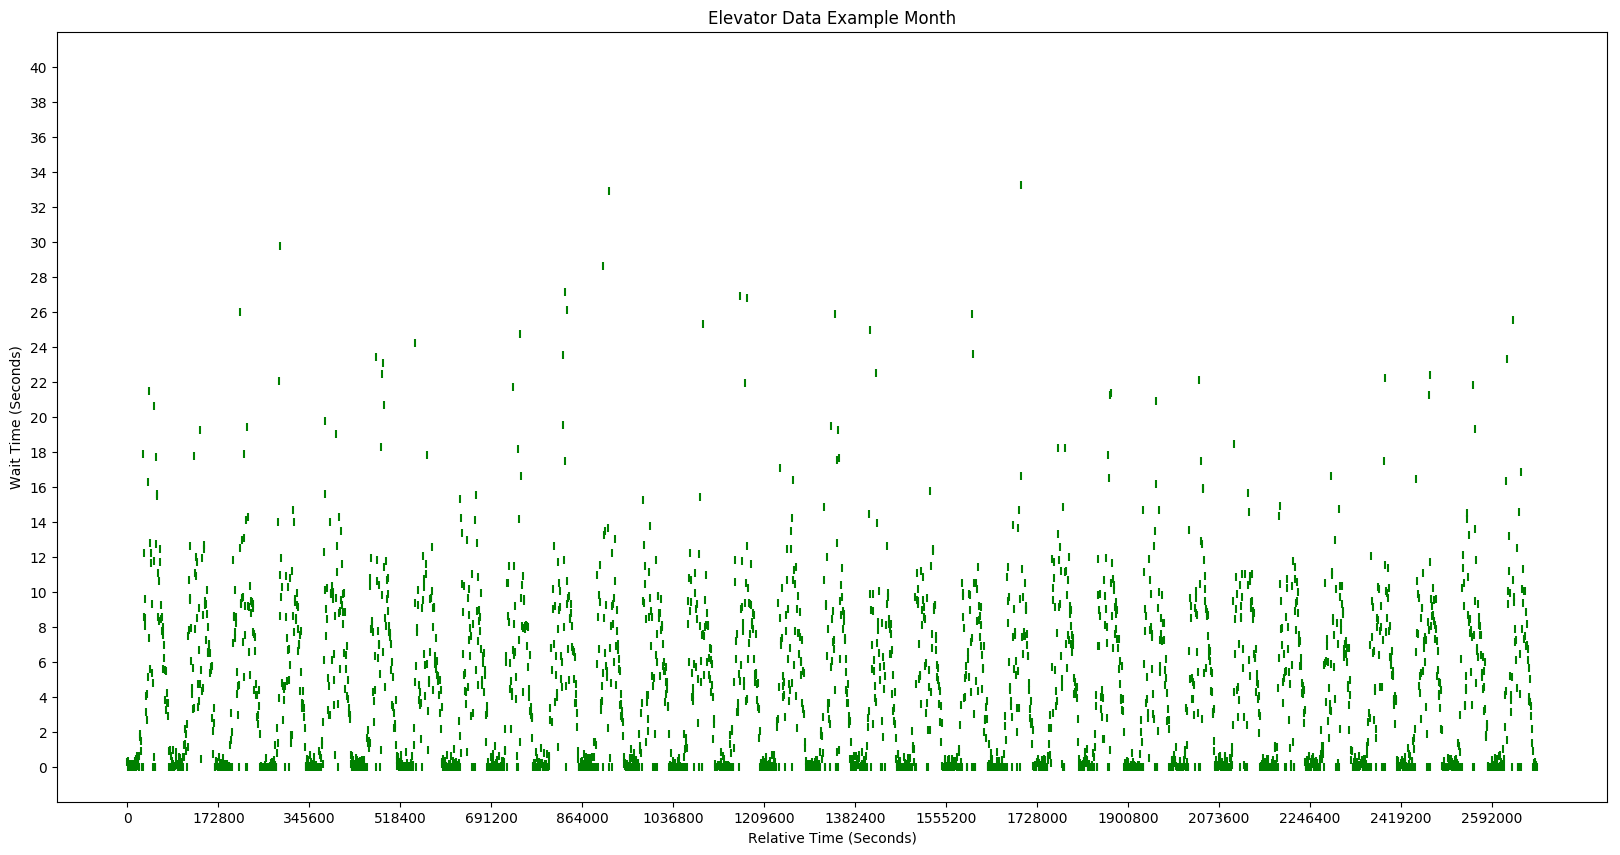
\includegraphics[width=\linewidth]{images/Elevator_Data_Example_Month.png}
    \caption{The training data for the first elevator month}
    \label{figure:Elevator Training Data}
  \end{figure}


  \subsection{ High Resolution Data }

  Finally, an additional data set has been included for comparison. During
  normal data generation observations are assumed to occur consistently ever
  15 minutes. In the additional ``High Resolution'' dataset, observations happen
  ever 1 minute. The inclusion of this additional dataset aims to outline how
  the models preform with larger sets of data while keeping the actual
  underlying data similar to the regular resolution dataset.

\end{document}
